\documentclass{article}
\textheight 23.5cm \textwidth 15.8cm
%\leftskip -1cm
\topmargin -1.5cm \oddsidemargin 0.3cm \evensidemargin -0.3cm
%\documentclass[final]{siamltex}

\usepackage{verbatim}
\usepackage{fancyhdr}
\usepackage{graphicx}

%\pagestyle{fancy} \lhead{FDM Homework Template} \chead{}
%\rhead{\bfseries Yan XU}
%
%\lfoot{} \cfoot{} \rfoot{\thepage}
%\renewcommand{\headrulewidth}{0.4pt}
%\renewcommand{\footrulewidth}{0.4pt}
%

%利用TEX排版系统的CTEX中文套装
\usepackage[UTF8,noindent]{ctex}
%等式对齐
\usepackage{amsmath}
\usepackage{amssymb}

\title{质点弹簧系统仿真}
\author{陈柯}

\begin{document}
	\maketitle
	
	\section{目的}
	
	实现弹簧质点模型的欧拉隐式方法及加速方法。
	
	\section{模拟方法}
	我们的问题是:如何由前 $n$ 帧信息,求得第 $n+1$ 帧信息(位移 $\boldsymbol x$,速
	度$\boldsymbol v$,时间间隔为$h$)?
	\subsection{欧拉隐式方法}
	欧拉隐式方法即以下两式:
	$$\boldsymbol x_{n+1}=\boldsymbol x_n+h\boldsymbol v_{n+1}$$
	$$\\\boldsymbol v_{n+1}=\boldsymbol v_n+h\boldsymbol M^{-1}
	(\boldsymbol f_{int}(t_{n+1}) +\boldsymbol f_{ext})$$
	其中$\boldsymbol M$为质点的质量矩阵。这里若假设三角网格网格共$N$个
	质点(顶点),那么这里的$\boldsymbol v_i,\boldsymbol x_i,\boldsymbol f$在实现的
	时候就是$3N\times 1$的矩阵。若记
	$$\boldsymbol y =\boldsymbol x_n + h\boldsymbol v_n + h^2\boldsymbol 
	M^{-1}\boldsymbol f_{ext}$$
	则有
	$$\boldsymbol M(\boldsymbol x_{n+1}-\boldsymbol y) 
	-h^2\boldsymbol f_{int}(\boldsymbol x_{n+1}) = 0$$
	为了解出$\boldsymbol x_{n+1}$,我们设
	\begin{equation}
		\boldsymbol g(\boldsymbol x) = \boldsymbol M(\boldsymbol x-\boldsymbol 
		y) -h^2\boldsymbol f_{int}(\boldsymbol x) \tag{*}
	\end{equation}
	利用Newton法进行以下的迭代:
	$$\boldsymbol x^{(k+1)}=\boldsymbol x^{(k)}-(\nabla \boldsymbol 
	g(\boldsymbol x^{(k)}))^{-1}\boldsymbol g(\boldsymbol x^{(k)})$$
	即可求解出$\boldsymbol x_{n+1}$。迭代初值可选为$\boldsymbol x^{(0)}=y$ 。实现过
	程当中,可规定当相邻两步之差小于某个值时就不再迭代。迭代得到位移$x$后需要更新速度
	$v_{n+1}=(x_{n+1}-x_{n})/h$。
	
	在质点弹簧系统中,上式中涉及关于弹力的求导,对于单个弹簧(端点为$\boldsymbol  
	x_1$,$\boldsymbol  x_2$),劲度系数为$k$,原长为$l$,$\boldsymbol x_1$所受弹力
	为
	$$\boldsymbol f(\boldsymbol x_1,\boldsymbol x_2)=k(||\boldsymbol 
	x_1-\boldsymbol x_2||-l)\frac{\boldsymbol x_2-\boldsymbol 
	x_1}{||\boldsymbol x_1-\boldsymbol x_2||}$$
	对其求导可得
	$$\frac{\partial\boldsymbol f}{\partial\boldsymbol x_1} 
	=k(\frac{l}{||\boldsymbol r||}-1)\boldsymbol 
	I-kl||\boldsymbol r||^{-3}\boldsymbol r \boldsymbol r^T,其中\boldsymbol 
	r=\boldsymbol x_1-\boldsymbol x_2,  \frac{\partial\boldsymbol f}{\partial 
	\boldsymbol x_2}=-\frac{\partial  \boldsymbol f}{\partial \boldsymbol 
	x_1}\\$$
	对所有弹簧求导并组装即可求得力的导数(组装为稀疏矩阵,矩阵为对称阵)。
	
	
	\subsection{加速方法(projective dynamic)}
	在上述欧拉方法中,对于内力(为保守力)有:
	$$\boldsymbol f_{int}(x)=-\nabla E(\boldsymbol x)$$
	故对方程$(*)$的求解可以转为为一个最小化问题:
	$$\boldsymbol x_{n+1}=\min\limits_{x}\frac{1}{2}(\boldsymbol x-\boldsymbol 
	y)^T\boldsymbol M(\boldsymbol x-\boldsymbol y)+h^2E(\boldsymbol x)$$
	同时对于弹簧的弹性势能可以描述为一个最小化问题:
	$$\frac{1}{2}k(||\boldsymbol p_1-\boldsymbol p_2||-r)^2=\frac{1}{2}k 
	\min\limits_{||\boldsymbol d||=r}||\boldsymbol p_1-\boldsymbol 
	p_2-\boldsymbol d||^2$$
	从而原问题转化为:
	$$\boldsymbol x_{n+1}=\min\limits_{x,\boldsymbol d\in\boldsymbol 
	U}\frac{1}{2}\boldsymbol x^T(\boldsymbol M+h^2\boldsymbol L)\boldsymbol 
	x-h^2\boldsymbol x^T\boldsymbol J \boldsymbol d-\boldsymbol x^T \boldsymbol 
	M \boldsymbol y	$$
	其中$$\boldsymbol U= \{ \boldsymbol d=(\boldsymbol d_1,\boldsymbol 
	d_2,...,\boldsymbol d_s),\boldsymbol d_s\in R^3,||\boldsymbol d_i||=l_i \} 
	(\mbox{$l_i$为第$i$个弹簧原长})$$
	$$\boldsymbol L=\left(\sum_{i=1}^{s}k_i\boldsymbol{A_i}\boldsymbol{A_i^T}
	\right)\otimes\boldsymbol{I_3}\in \mathbb{R}^{3m\times 3m}$$
	$$\boldsymbol J=\left(\sum_{i=1}^{s}k_i\boldsymbol{A_i}\boldsymbol{S_i^T}
	\right)\otimes\boldsymbol{I_3}\in \mathbb{R}^{3m\times 3s}$$
	$\boldsymbol{A_i}$为第$i$个弹簧的Incidence 
	Vector,即$A_{i,i_1}=1,A_{i,i_2}=-1$,其余均为0。类似地,$\boldsymbol{S_i}\in
	\mathbb{R}^{s}$为第$i$个弹簧indicator,即$S_{i,j}=\delta_{i,j}$。矩阵
	$\boldsymbol{L}$不过是以劲度系数为权重的质点弹簧系统的Laplace矩阵。从而可以对 
	$\boldsymbol x$,$\boldsymbol d$ 迭代优化求得该优化问题的解:
	$$\mbox{先对$\boldsymbol{x}$优化:求解方程}
	(\boldsymbol{M}+h^2\boldsymbol {L})\boldsymbol{x}=h^2\boldsymbol{J} 
	\boldsymbol{d}+\boldsymbol{M}\boldsymbol{y}$$
	$$\mbox{再更新$\boldsymbol{d}$:}
	\boldsymbol d_i=l_i\frac{\boldsymbol p_{i_1}-\boldsymbol 
	p_{i_2}}{||\boldsymbol p_{i_1}-\boldsymbol p_{i_2}||}$$
	这里$l_i$为第$i$个弹簧原长,$\boldsymbol p_{i_1},\boldsymbol p_{i_2}$
	为其两端点。重复迭代过程直到收敛。
	\subsection{边界条件和约束}
	通常模拟过程中物体会有各种约束或额外条件,例如物体被固定了几个点,对某些点施加外力(
	如重力、浮力、风力等)。
	\subsubsection{外力条件}
	1.物体受到的外力可以直接加在模拟的外力项中,其导数为0.
	
	2.对于重力,可以将其加在外力中,另一方面,重力为保守力,也可以将重力势能加在能量项
	中与弹性势能进行合并
	\subsubsection{位移约束}
	这里主要考虑固定部分质点的情形,有两种方法处理:
	
	1.第一种方法是在每一帧中求出该点的内力,再施加与该内力大小相同,方向相反的外力,但
	与上一种情形不同的是,若该内力对位移导数不为 0,则该外力对位移导数也不为 0,需要将
	其导数考虑进去;
	
	2.第二种方法为仅考虑真正的自由坐标,降低问题的维数,具体如下:
	
	若考虑固定点,将所有m个质点的坐标列为列向量 $x\in R^{3m}$,将所有n 
	个自由质点坐标(无约束坐标)列为列向量 $x_f\in R^{3n}$,则两者关系:
	$$\boldsymbol x_f=\boldsymbol K\boldsymbol x$$
	$$\boldsymbol x=\boldsymbol K^T\boldsymbol x_f+\boldsymbol b,$$
	其中 $K\in R^{3n\times 3m}$ 为单位阵删去约束坐标序号对应行所得的稀疏矩阵,$b$ 为
	与约束位移有关的向量,计算为 $b=x-K^TKx$, 若约束为固定质点则 $b$ 为常量。由此我们
	将原本的关于 $x$ 的优化问题转化为对 $x_f$ 的优化问题:欧拉隐式方法中求解方程为:
	$$\boldsymbol g_1(\boldsymbol x_f) = K(\boldsymbol M(\boldsymbol 
	x-\boldsymbol y) -h^2\boldsymbol f_{int}(\boldsymbol x)) = 0$$
	$$\mbox{梯度:}\nabla_{x_f} \boldsymbol g_1(\boldsymbol x_f) = 
	K\nabla_{x} \boldsymbol g(\boldsymbol x)K^T$$
	加速方法中优化问题中 $x$ 迭代步骤转化为求解关于 $x_f$ 的方程:
	$$K(\boldsymbol M+h^2\boldsymbol L)K^T\boldsymbol x_f=K(h^2\boldsymbol J 
	\boldsymbol d+ \boldsymbol M \boldsymbol y-(\boldsymbol M+h^2\boldsymbol 
	L)\boldsymbol b)$$
	\section{实现结果}
	实现结果请看随本报告附带的视频。
	\subsection{迭代停止的条件}
	我两种方法在求解过程中,都采用了这样的判断迭代停止的条件:前后迭代差距小于1e-5或迭
	代次数大于5时,就停止迭代,结果作为本次步长的结果。
	\clearpage
	\subsection{交互}
	我实现了以下的交互:
	\begin{figure}[htb]
		\begin{center}
			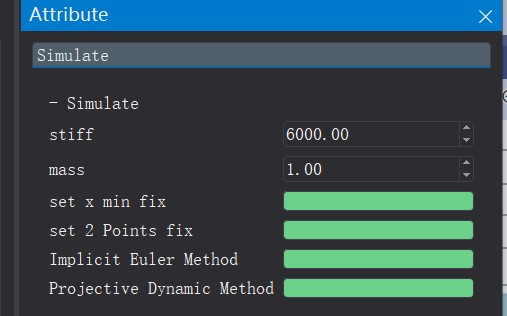
\includegraphics[width=4in]{ui.jpg}
		\end{center}
	\end{figure}

	用户可以控制每根弹簧的劲度系数,每个质点的质量,仿真的方法,以及固定点的确定。这里
	可以固定2个点,或者所有x坐标最小的点。
	\subsection{结果评估}
	我们会发现:
	
	1.一旦质点数增加,欧拉隐式方法的劣势就特别明显了,计算速度相当慢;而[1]提出的加速方
	法就算在441个质点的稠密网格上计算速度也很快,仿真效果很不错。
	
	2.我们实现的算法就是对质点弹簧系统适用的,所以算法可以直接对四面体网格执行,不仅仅
	对曲面片网格适用。
\section{参考文献}
  $[1]$Tiantian Liu, et al. "Fast simulation of mass-spring systems." *Acm 
  Transactions on Graphics (Pro. Siggraph Asia)* 32.6(2013):1-7.
\end{document}
